\documentclass{beamer}
\usepackage[slovene]{babel}
\usepackage[utf8]{inputenc}
\usepackage[T1]{fontenc}
\usepackage{array}
\usepackage{url}
\usepackage{amsmath} 
\usepackage{amsthm}  
\usepackage{amssymb} 
\usepackage{graphicx}
\usepackage{tikz}



% ===================================================================
\usetheme{Berlin}
\usecolortheme{default}
\usepackage{palatino}
\usefonttheme{serif}
\useoutertheme{infolines}
\useinnertheme[shadows]{rounded}
\beamertemplatenavigationsymbolsempty



\author{Urh Primožič}
\title[O Beamerju in zaka je lajf]{Priprava prosojnic v \LaTeX{}-u}
\subtitle{Uporaba paketa beamer}
\institute[FMF]{Fakulteta za matematiko in fiziko}
\date{}


\newtheorem{izrek}{Izrek}
\newtheorem{definicija}{Definicija}
\newtheorem*{dokaz}{Dokaz}
%%%%%%%%%%%%%%%%%%%%%%%%%%%%%%%%%%%%%%%%%%%%%%%%%%%%%%%%%%
\begin{document}

\frame{\titlepage}
% -------------------------------------------------------------------


\begin{frame}
      \frametitle{Kratek pregled}
      \tableofcontents[pausesections]
\end{frame}

% ===================================================================



\section{Razporeditev vsebine}


% -------------------------------------------------------------------

 
 \begin{frame}
      \frametitle{Naštevanje}
      Za naštevanje lahko uporabimo okolje \texttt{itemize}:         
         \begin{itemize}
            \item Prva točka.
            \item Druga točka.
            \item Tretja točka.
         \end{itemize}
      ali pa okolje \texttt{enumerate}:
\begin{enumerate}
            \item Prva točka.
            \item Druga točka.
            \item Tretja točka.
\end{enumerate}
   
 \end{frame}
% -------------------------------------------------------------------

 
 \begin{frame}
      \frametitle{Bloki z naslovom}
      Dele besedila lahko zapišemo v bloke.\\
      Uporabimo okolja \texttt{block}, \texttt{exampleblock}, \texttt{alertblock}.\\
      Za parameter okolja napišemo naslov bloka.
      \begin{block}{Opomba}
      Tako je videti block z naslovom.
      \end{block}
      \begin{exampleblock}{Primer}
         Tako je videti \texttt{exampleblock} z naslovom.
      \end{exampleblock}
      \begin{alertblock}{Opozorilo}
         Tako je videti \texttt{alertblock} z naslovom.
      \end{alertblock}
 \end{frame}

% -------------------------------------------------------------------


\begin{frame}
      \frametitle{Bloki brez naslova}
      Blok lahko ima tudi prazen naslov.
      \\V takem primeru bo brez naslovne vrstice.         
         \begin{block}

            Tako je videti \texttt{block} s praznim naslovom.
         \end{block}         
         \begin{exampleblock}

            Tako je videti \texttt{exampleblock} s praznim naslovom.
         \end{exampleblock}      
         \begin{alertblock}

            Tako je videti \texttt{alertblock} s praznim naslovom.
         \end{alertblock}
\end{frame}

% -------------------------------------------------------------------


\begin{frame}
      \frametitle{Stolpci}

\begin{columns}
         \column{0.5\textwidth}
            \begin{itemize}         
                        \item Besedilo lahko pišemo v več stolpcih.
                        \item Osnovno okolje je \texttt{columns}.
                        \item Posamezen stolpec opišemo v okolju \texttt{column}.
                        \item Vsebina stolpca je lahko poljubna.
                        \item Za primer imamo v desnem stolpcu napis v bloku in sliko sončnice.                        
            \end{itemize}
         \column{0.5\textwidth}
         \begin{exampleblock}
            
            Slika v stolpcu.
         \end{exampleblock}
         \begin{figure}
            \includegraphics{soncnica.jpg}
         \end{figure}
\end{columns}
\end{frame}

% ===================================================================

\section{Matematične trditve}

% -------------------------------------------------------------------

   
   \begin{frame}
      \frametitle{Praštevila}
        
        \begin{definicija}
            Praštevilo je naravno število, ki ima natanko dva delitelja.
        \end{definicija}

\begin{exampleblock}{Zgledi}                        
               \begin{itemize}
                  \item 1 je praštevilo (ima samo enega delitelja: 1).
                  \item 2 je praštevilo (ima dva delitelja: 1 in 2).
                  \item 3 je praštevilo (ima dva delitelja: 1 in 3).
                  \item 4 ni praštevilo (ima tri delitelje: 1, 2 in 4).
               \end{itemize}
\end{exampleblock}
   \end{frame}

% -------------------------------------------------------------------


\begin{frame}
      \frametitle{Praštevila}
         
         \begin{izrek}
            Praštevil je neskončno mnogo.
         \end{izrek}
         
         \begin{block}
            Denimo, da je praštevil končno mnogo.               
               \begin{itemize}
                  \item Naj bo $p$ največje praštevilo.
                  \item Naj bo $q$ produkt števil $1, 2, \ldots, p$.
                  \item Število $q+1$ ni deljivo z nobenim praštevilom, torej je $q+1$ praštevilo.
                  \item To je protislovje, saj je $q+1>p$.
               \end{itemize}
         \end{block}
\end{frame}

% ===================================================================

\section{Postopno odkrivanje vsebine}

% -------------------------------------------------------------------

   
   \begin{frame}
      \frametitle{Konstrukcija pravokotnice na premico p skozi točko T}
              
              \begin{columns}
                 
                 \begin{column}{0.5\textwidth}
                    \begin{itemize}
                        \item<1-> Dani sta premica p in točka T.
                        \item<2-> Nariši lok k s središčem v T.
                        \item<3-> Premico p seče v točkah A in B.
                        \item<4-> Nariši lok m s središčem v A.
                        \item<5-> Nariši lok n s središčem v B in z enakim polmerom.
                        \item<6-> Loka se sečeta v točki C.
                        \item<7-> Premica skozi točki T in C je pravokotna na p.
                    \end{itemize}
                 \end{column}
               \begin{column}{0.5\textwidth}
                     \centering
                     \includegraphics<1>[width=0.95\textwidth]{pic1}
                     \includegraphics<2>[width=0.95\textwidth]{pic2}
                     \includegraphics<3>[width=0.95\textwidth]{pic3}
                     \includegraphics<4>[width=0.95\textwidth]{pic4}
                     \includegraphics<5>[width=0.95\textwidth]{pic5}
                     \includegraphics<6>[width=0.95\textwidth]{pic6}
                     \includegraphics<7>[width=0.95\textwidth]{pic7}
               \end{column}
              \end{columns}
            
   \end{frame}

% -------------------------------------------------------------------


\begin{frame}
      \frametitle{Odkrivanje tabele po vrsticah}

\begin{tabular}{c|c c c c}
            Oznaka & A & B & C & D \\ \hline
            \onslide<2-> X & 1 & 2 & 3 & 4 \\
            \onslide<3-> Y & 3 & 4 & 5 & 6 \\
            \onslide<4-> Z & 5 & 6 & 7 & 8
\end{tabular}
\end{frame}

% -------------------------------------------------------------------

\begin{frame}
   \frametitle{Odkrivanje tabele po stolpcih}

\begin{tabular}{c | >{\onslide<2->}c >{\onslide<3->}c >{\onslide<4->}c >{\onslide<5->}c <{\onslide}}
         Oznaka & A & B & C & D \\ \hline
         X & 1 & 2 & 3 & 4 \\
         Y & 3 & 4 & 5 & 6 \\
         Z & 5 & 6 & 7 & 8
\end{tabular}
\end{frame}

% ===================================================================

\subsection{Razno}

% -------------------------------------------------------------------
\begin{frame}
   \centering
   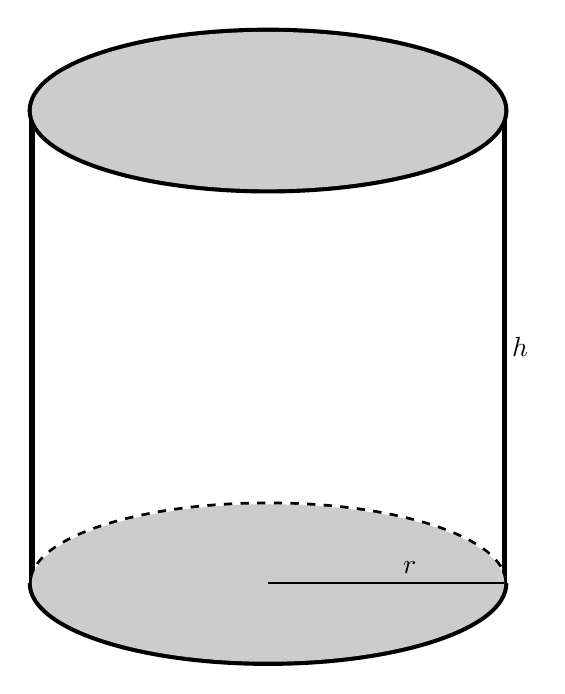
\begin{tikzpicture}
       \draw[line width = 2pt] (3,-1) -- (3,5);
       \draw[line width = 2pt] (-3,-1) -- (-3,5);
       \draw[line width = 3pt] (0,5) ellipse (3 and 1);
       \draw[line width = 2pt, dashed] (3,-1) arc  (0:180:3 and 1);
       \draw[line width = 3pt] (-3,-1) arc  (180:360:3 and 1);
\pause
      \begin{scope}[color=black!20]
         \fill[line width = 1pt] (0,5) ellipse (3 and 1);
         \fill[line width = 1pt] (0,-1) ellipse (3 and 1);
      \end{scope}
      \pause
      \node at (3.2,2) {$h$};
      \node at (1.8,-0.8) {$r$};
      \draw[line width = 1pt] (0,-1) -- (3, -1);

      
      \end{tikzpicture}
\end{frame}
% ===================================================================

\end{document}
%%DONE 12.11.2019 14:43